\documentclass[12pt,a4paper]{report}
\usepackage[utf8]{inputenc}
\usepackage[utf8]{vietnam} %Bien dich duoc tieng Viet
\usepackage{amsmath,amsfonts,amssymb} %Font toan
\usepackage{type1cm}
\usepackage{graphicx}
\graphicspath{ {images/} }
\usepackage{subfig}
\usepackage[unicode]{hyperref} %Tu dong tao bookmark
\usepackage{indentfirst} %Thut vao dau dong o tat ca cac doan
\usepackage{listings} %Dinh dang code
\usepackage{color} %Mau sac
\usepackage[left=2.5cm,right=1.5cm,top=1.5cm,bottom=1.5cm]{geometry} %Canh lề trái - phải - trên - dưới cho tài liệu
\definecolor{dkgreen}{rgb}{0,0.6,0}
\definecolor{gray}{rgb}{0.5,0.5,0.5}
\definecolor{mauve}{rgb}{0.58,0,0.82}

\lstset{frame=tb,
  language=C,
  aboveskip=3mm,
  belowskip=3mm,
  showstringspaces=false,
  columns=flexible,
  basicstyle={\small\ttfamily},
  numbers=left,
  numberstyle=\tiny\color{gray},
  keywordstyle=\color{blue},
  commentstyle=\color{dkgreen},
  stringstyle=\color{mauve},
  breaklines=true,
  captionpos=t,
  breakatwhitespace=true,
  tabsize=2
}
\begin{document}
%\input{title-page.tex}
%\input{install-pi/Install-Pi-OS.tex}
\tableofcontents
\chapter{Điều khiển và sao chép dữ liệu với Raspberry Pi}
%Có một cách có thể dùng để điều khiển Raspberry Pi
\section{Điều khiển bằng cách kết nối trực tiếp với màn hình, bàn phím và chuột}
\begin{itemize}
\item \textit{Điều khiển}: Kết nối chuột và bàn phím qua các cổng USB. Với màn hình thông thường có 2 loại: màn hình hỗ trợ cổng HDMI và màn hình hổ trợ cổng VGA.
\item \textit{Sao chép dữ liệu}: Sử dụng USB.
\end{itemize}
\subsection{Màn hình hổ trợ cổng HDMI}
Ta kết nối màn hình qua cable HDMI. Có thể bạn sẽ cần tùy chỉnh một số thông sau cho phù hợp:
\subsection{Màn hình hổ trợ cổng VGA}
Để hiển thị được, ta cần có cable chuyển đồi từ VGA sang HDMI.
\section{Điều khiển bằng giao tiếp nối tiếp thông qua cổng RS232}
\begin{itemize}
\item Thực hiện kết nối Pi và module RS232 như sau:
\begin{center}
\begin{tabular}{c|c}
Pi & RS232\\ \hline
3.3V & VCC\\
TX & TX \\ 
RX & RX\\
GND & GND
\end{tabular}
\end{center}
\item Cài đặt gói phần mềm \verb|screen|: \verb|sudo apt-get install screen| trên máy tính Ubuntu.
\item Chạy lệnh sau: \verb|sudo screen /dev/ttyUSB0 115200|
\item Thực hiện xong lệnh trên, ta nhấn Enter một lần nữa để kết nối với Pi.
\item Nhập username và password để đăng nhập.
\item Sao chép dữ liệu: dùng USB.
\item[$\ast$] Ta có thể dùng Putty (trên hệ điều hành Window) để điều khiển: chọn \verb|Serial|, điền vào khung \verb|Serial line| tên cổng (ví dụ: COM1, COM2,\ldots), trong khung \verb|Speed| điền tốc độ là \verb|115200|. Nhập username và password để đăng nhập.
\end{itemize}
\section{Điều khiển từ xa khi Raspberry Pi có kết nối mạng}
Khi Raspberry Pi có kết nối mạng Internet, ta có thể dùng các phần mềm: \verb|SSH|, \verb|Remote Desktop|, \verb|VNC|,\ldots~ để điều khiển.
\begin{itemize}
\item Kiểm tra địa chỉ IP của Pi bằng phần mềm: ipscan (trên Windows) hoặc nmap (trên Ubuntu).
\item Chọn chương trình phù hợp để điều khiển Raspberry Pi: 
\begin{itemize}
\item Với \verb|SSH|: không hổ trợ giao diện đồ họa.
\item Với \verb|Remote Desktop| (Pi cần cài đặt: \verb|xrdp|, dùng lệnh: \verb|sudo apt-get install xrdp|), \verb|VNC|: có hổ trợ giao diện đồ họa.
\end{itemize}
\item Tùy theo chương trình bạn chọn: ta cần phải nhập địa chỉ IP, username và password (nếu có yêu cầu điền số \verb|port|: ta điền 22).
\item Sao chép dữ liệu:
\begin{itemize}
\item Trên Window: dùng \verb|Winscp|.
\item Trên Ubuntu: dùng \verb|FileZilla|.
\item[$\ast$] Ta cũng cần nhập vào thông tin như trên để truy cập được Pi.
\end{itemize}
\item \textit{Lưu ý}: Phần trình bày trên áp ngay cho mạng nội bộ, khi không phải mạng nội bộ ta cần cấu hình mạng rồi mới áp dụng được hướng dẫn ở phần này.
\end{itemize}


\chapter{Mạng Internet với Raspberry Pi}
\section{Kết nối internet với dây mạng LAN}
Trên Raspberry Pi có hổ trợ cổng Ethernet, chúng ta có thể kết nối dây mạng trực tiếp vào đây.
\section{Kết nối internet với USB Wifi}
Trong phần này, mình sử dụng USB Wifi TP Link 725N
\subsection{Cài đặt Drive}
Tham khảo tại: \verb|https://www.raspberrypi.org/forums/viewtopic.php?p=462982|

Thực hiện theo các bước sau:
\begin{itemize}
\item Xác định phiên bản hệ điều hành Raspbain:
\begin{lstlisting}[language=make]
$ uname -a
Linux raspberrypi 4.1.13+ #826 PREEMPT Fri Nov 13 20:13:22 GMT 2015 armv6l GNU/Linux
\end{lstlisting}
Trong ví dụ trên, phiên bản hệ điều hành là \verb|4.1.13+ #826|. 
\item Vào địa chỉ bên dưới để tải drive:

\verb|https://www.raspberrypi.org/forums/viewtopic.php?p=462982|
\item Cài đặt drive, thực hiện các lệnh bên dưới:
\begin{lstlisting}[language=make]
wget https://dl.dropboxusercontent.com/u/80256631/8188eu-201xyyzz.tar.gz
tar -zxvf 8188eu-201xyyzz.tar.gz
sudo install -p -m 644 8188eu.ko /lib/modules/$(uname -r)/kernel/drivers/net/wireless
sudo insmod /lib/modules/$(uname -r)/kernel/drivers/net/wireless/8188eu.ko
sudo depmod -a
\end{lstlisting}
Đối với Raspberry Pi 2, chúng ta chỉ cần thực hiện 2 lệnh sau:
\begin{lstlisting}[language=make]
tar xzf 8188eu-2015yyzz.tar.gz
./install.sh
\end{lstlisting}
Với \verb|8188eu-201xyyzz.tar.gz| là drive phù hợp với phiên bản hệ điều hành của bạn.

Bạn có thể tải drive từ máy tính rồi chép vào Raspberry Pi để cài đặt (cách này dùng cho Pi chưa được kết nối với Internet).
\item[$\ast$] Trong quá trình cập nhật các phiên bản mới của hệ điều hành, khi đó Raspberry Pi không còn nhận USB Wifi nữa, lúc đó ta cần cài đặt Drive mới cho USB Wifi.
\end{itemize}
\subsection{Cài đặt địa chỉ IP tĩnh}
Tham khảo tại địa chỉ: 

\begin{footnotesize}
\verb|http://weworkweplay.com/play/automatically-connect-a-raspberry-pi-to-a-wifi-network/|
\end{footnotesize}\\

Ta sửa đổi nội dung của 2 tập tin dưới đây:
\begin{itemize}
\item Tập tin: \verb|interfaces|, mở tập tin:
\begin{lstlisting}[language=bash]
$ sudo nano /etc/network/interfaces
\end{lstlisting}
và thay đổi nội dung như sau:
\lstinputlisting[language=make]{interfaces}
\item Tập tin: \verb|wpa_supplicant.conf|,  mở tập tin:
\begin{lstlisting}[language=bash]
$ sudo nano /etc/wpa_supplicant/wpa_supplicant.conf
\end{lstlisting}
và thay đổi nội dung như sau:
\lstinputlisting[language=make]{wpa_supplicant.conf}
\end{itemize}
\section{Sử dụng chung Wifi với Laptop}
Ta kết nối cổng Ethernet của Pi và Laptop với nhau. Sử dụng tín năng Share Wifi trên Laptop:
\subsection{Hệ điều hành Ubuntu}
Thực hiện theo các bước sau:
\begin{itemize}
\item Trong thanh tìm kiếm \verb|Dash|: gõ vào \verb|Network Connections|, chọn \verb|Network Connections| để mở lên.
\begin{figure}[!h]
\begin{center}
{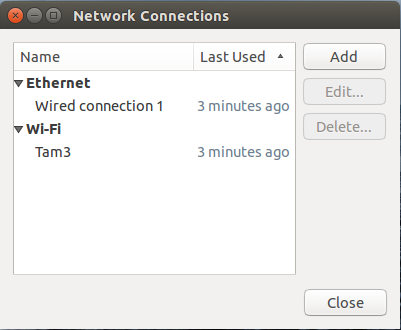
\includegraphics[scale=.5]{network/images/share-wifi-1}}
\end{center}
\caption{Mở \textsf{Network Connections}}
\end{figure}
\item Chọn \verb|Add|:
\begin{figure}[!h]
\begin{center}
{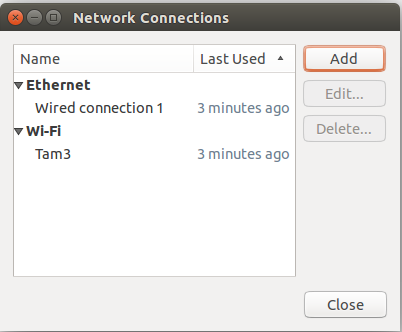
\includegraphics[scale=.5]{network/images/share-wifi-2}}
\end{center}
\caption{Chọn \textsf{Add}}
\end{figure}
\newpage
\item Chọn \verb|Create|:
\begin{figure}[!h]
\begin{center}
{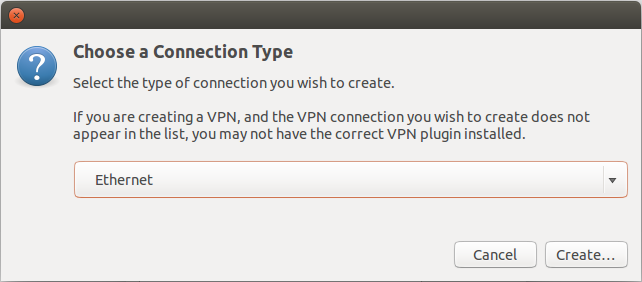
\includegraphics[scale=.4]{network/images/share-wifi-3}}
\end{center}
\caption{Chọn \textsf{Create\ldots}}
\end{figure}
\item Điền tên trong ô \verb|Connection name|:
\begin{figure}[!h]
\begin{center}
{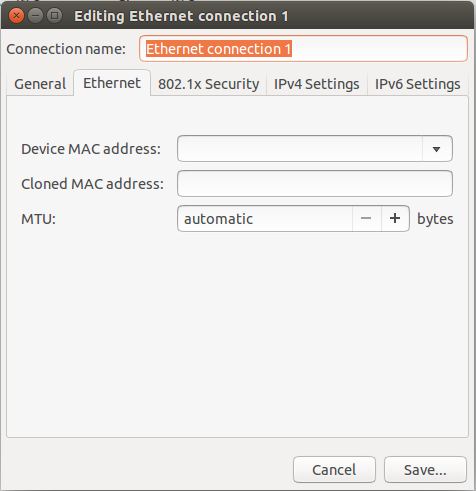
\includegraphics[scale=.4]{network/images/share-wifi-4}}
\caption{Điền tên trong ô \textsf{Connection name}}
\end{center}
\end{figure}
\item Chọn tab \verb|IPv6 Settings|, chọn \verb|Method| là \verb|Automactic|:
\begin{figure}[!h]
\begin{center}
{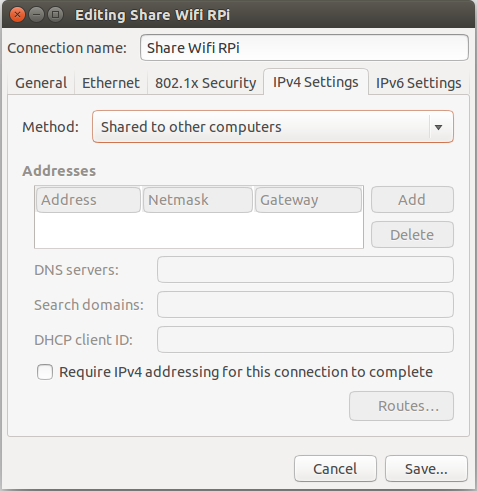
\includegraphics[scale=.4]{network/images/share-wifi-5}}
\caption{Chọn tab \textsf{IPv6 Settings}, chọn \textsf{Method} là \textsf{Automactic}}
\end{center}
\end{figure}
\item Chọn tab \verb|IPv4 Settings|, chọn \verb|Method| là \verb|Share to orther computers|:
\begin{figure}[!h]
\begin{center}
{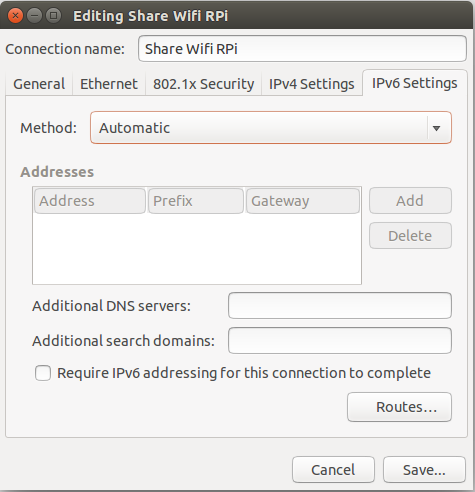
\includegraphics[scale=.5]{network/images/share-wifi-6}}
\caption{Chọn tab \textsf{IPv6 Settings}, chọn \textsf{Method} là \textsf{Share to orther computers}}
\end{center}
\end{figure}
\item Chọn \verb|Save| rồi chọn \verb|Close|.
\item Mở cửa sổ lệnh \verb|Terminal| gõ lệnh:
\begin{lstlisting}[language=bash]
$ sudo cat /var/lib/misc/dnsmasq.leases
1461927547 b8:27:eb:6a:bf:9a 10.42.0.31 raspberrypi ff:eb:6a:bf:9a:00:01:00:01:1c:dd:60:6b:b8:27:eb:6a:bf:9a
\end{lstlisting}
\item Địa chỉ của Pi lúc này là \verb|10.42.0.31|
\item Truy cập qua SSH bằng lệnh:
\begin{lstlisting}[language=bash]
$ ssh pi@10.42.0.31
\end{lstlisting}
\item Nhập password đăng nhập tài khoản username là \verb|pi|.
\end{itemize}
\chapter{Tự động đăng nhập Raspberry Pi sau khi khởi động}
\label{Sub:auto-login}
Tham khảo tại:

\begin{footnotesize}
\verb|http://www.raspberrypi-spy.co.uk/2015/02/how-to-autorun-a-python-script-on-raspberry-pi-boot/|
\end{footnotesize}

Mặc định khi Raspberry Pi khởi động, cần phải đăng nhập username và password mới sử dụng được. Với một số ứng dụng thực tế, cần tự động đăng nhập mới có thể hoạt động được.\\

Thực hiện theo các bước sau:
\begin{itemize}
\item Mở file \verb|inittab|, dùng lệnh:
\begin{lstlisting}[language=bash]
$ sudo nano /etc/inittab
\end{lstlisting}
\item Tìm đến dòng dưới và thêm dấu \verb|#| vào trước nó:
\begin{lstlisting}[language=bash]
1:2345:respawn:/sbin/getty 115200 tty1
\end{lstlisting}
(tìm đến dòng có \verb|1:2345:respawn:/sbin/getty ....| là được, còn các tham số phía sau tùy thuộc vào phiên bản hệ điều hành).
\item Thay thế dòng trên bằng dòng sau (với \verb|pi| là tên username):
\begin{lstlisting}[language=bash]
1:2345:respawn:/bin/login -f pi tty1 </dev/tty1 >/dev/tty1 2>&1
\end{lstlisting}
\item Nhấn \verb|Ctrl - X - Y| để lưu lại nội dung thay đổi và thoát.
\item Khởi động lại Pi: \verb|sudo reboot|.
\end{itemize}
\chapter{Chạy chương trình Python trên Raspberry Pi}
\section{Python trên Raspberry Pi}\label{run-python}
Ta phân biệt theo 2 trường hợp sau:
\begin{itemize}
\item Chạy các lệnh không liên quan đến phần cứng là các chân GPIO, ta sẽ gõ các lệnh sau:
\begin{itemize}
\item Chạy ở chế độ dòng lệnh:
\begin{lstlisting}[language=bash]
$ python
\end{lstlisting}
\item Khi đã có sẳn một file \verb|.py| (ví dụ: \verb|file.py|):
\begin{lstlisting}[language=bash]
$ python file.py
\end{lstlisting}
\end{itemize}
\item Các lệnh liên quan đến phần cứng can thiệp vào các chân GPIO hoặc cần quyền root, ta phải chạy với quyền root: dùng \verb|sudo python| hoặc \verb|sudo python file.py| (cách dùng 2 lệnh này giống như trên).
\end{itemize}
\section{Tự động chạy một chương trình python sau khi Reboot}
Ở phần~\ref{run-python}, ta phải thực hiện đánh lệnh thì file python mới được gọi, với nhiều ứng dụng tự động, cần tự động chạy chương trình python sau khi reboot. Ta có một số cách sau:

Ví dụ, ta cần chạy file python có tên là \verb|myfile.py|.
\subsection{Sử dụng cron}
Tham khảo tại: \verb|https://www.youtube.com/watch?v=8iU9TnYFOV0|\\
Thực hiện theo các bước sau:
\begin{itemize}
\item Không cần tự động đăng nhập.
\item Copy file \verb|myfile.py| đến thư mục \verb|\home\pi| (dùng lệnh \verb|cp|).
\item Mở file \verb|crontab| gõ lệnh:
\begin{lstlisting}[language=bash]
$ sudo crontab -e
\end{lstlisting}
\item Thêm dòng sau vào cuối file: 
\begin{lstlisting}[language=bash]
@reboot sudo python myfile.py &
\end{lstlisting}
Ký hiệu \verb|&| có nghĩa là file \verb|myfile.py| sẽ chạy nền.
\begin{figure}[h!]
\begin{center}
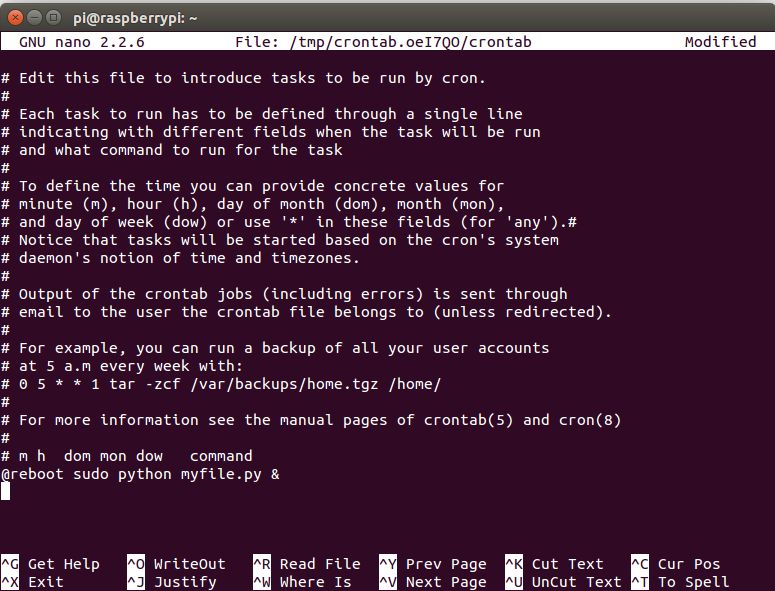
\includegraphics[scale=.5]{run-script-python/images/auto-run-python-1}
\end{center}
\end{figure}
\item Nhấn \verb|Ctrl - X - Y| để lưu lại nội dung thay đổi và thoát.
\item Khởi động lại Pi: \verb|sudo reboot|.
\end{itemize}
Nói thêm về \verb|cron|\footnote{\textsf{https://embeddedday.com/projects/raspberry-pi/a-step-further/running-python-script-at-boot/}} \verb|cron| là một lịch trình, được khai báo với cú pháp sau:
\begin{lstlisting}[language=bash]
1 2 3 4 5 /path/to/command arg1 arg2
\end{lstlisting}
Ý nghĩa của các tham số:
\begin{itemize}
\item \verb|1 = Minutes (0 – 59)|
\item \verb|2 = Hours (0 – 23)|
\item \verb|3 = Days (0 – 31)|
\item \verb|4 = Month (0 – 12)|
\item 5 = Day of the week (0 – 7) (Sunday is the 0 day)|
\end{itemize}
Ta có thể thay thế 1 trong 5 tham số trên bằng các tham số dưới đây:
\begin{itemize}
\item \verb|@reboot|	= Run once, at startup.
\item \verb|@yearly|	= Run once a year
\item \verb|@monthly| = Run once a month
\item \verb|@weekly|	= Run once a week
\item \verb|@daily| = Run once a day
\item \verb|@midnight| = Pretty much the same as \verb|@daily|
\item \verb|@hourly|	= Run once an hour
\end{itemize}
\subsection{Sử dụng profile}
Tham khảo tại:

\begin{footnotesize}
\verb|http://www.raspberrypi-spy.co.uk/2015/02/how-to-autorun-a-python-script-on-raspberry-pi-boot/|
\end{footnotesize}

Thực hiện theo các bước sau:
\begin{itemize}
\item Làm cho Pi có thể tự động đăng nhập được (xem \textit{chủ đề \ref{Sub:auto-login} trang \pageref{Sub:auto-login}}).
\item Mở file profile, dùng lệnh: 
\begin{lstlisting}[language=bash]
$ sudo nano /etc/profile
\end{lstlisting}
\item Kéo xuống dòng cuối dòng, thêm nội dụng sau vào file:
\begin{lstlisting}[language=bash]
sudo python /home/pi/myfile.py &
\end{lstlisting}
Ký hiệu \verb|&| có nghĩa là file \verb|myfile.py| sẽ chạy nền.
\item Nhấn \verb|Ctrl - X - Y| để lưu lại nội dung thay đổi và thoát.
\item Khởi động lại Pi: \verb|sudo reboot|.
\end{itemize}
\subsection{Sử dụng cron kết hợp với tạo file .sh}
Tham khảo tại:

\begin{footnotesize}
\verb|http://www.instructables.com/id/Raspberry-Pi-Launch-Python-script-on-startup/?ALLSTEPS|
\end{footnotesize}

Thực hiện theo các bước sau:
\begin{itemize}
\item Tạo một \verb|.sh| (ví dụ: launcher.sh):
\begin{lstlisting}[language=bash]
$ nano launcher.sh
\end{lstlisting}
\item Nội dung file như sau (thay đổi nội dung của ví dụ cho phù hợp):
\begin{lstlisting}[language=bash]
#!/bin/sh
# launcher.sh
# navigate to home directory, then to this directory, then execute python script, then back home

cd /
cd home/pi/bbt  #thu muc chua file .py
sudo python bbt.py #Lenh chay file python
cd /
\end{lstlisting}
Nhấn \verb|Ctrl - X - Y| để lưu và thoát.
\item Làm cho file \verb|.sh| trở thành file thực thi (executable): 
\begin{lstlisting}[language=bash]
$ chmod 755 launcher.sh
\end{lstlisting}
\item Kiểm tra file \verb|.sh| ta vừa tạo có thực thi được không:
\begin{lstlisting}[language=bash]
$ sh launcher.sh
\end{lstlisting}
\item Tạo thư mục \verb|logs| trong thư mục \verb|\home\pi|:
\begin{lstlisting}[language=bash]
$ cd ~
$ mkdir logs
\end{lstlisting}
\item Mở \verb|crom|:
\begin{lstlisting}[language=bash]
$ sudo crontab -e
\end{lstlisting}
\item Thêm file \verb|.sh| vào \verb|cron|:
\begin{lstlisting}[language=bash]
@reboot sh /home/pi/bbt/launcher.sh >/home/pi/logs/cronlog 2>&1
\end{lstlisting}
Nhấn \verb|Ctrl - X - Y| để lưu và thoát.
\item Khởi động lại Pi: \verb|sudo reboot|
\end{itemize}
\end{document}